% PRL look and style (easy on the eyes)
\RequirePackage[hyphens]{url}
\documentclass[aps,pre,twocolumn,nofootinbib,superscriptaddress,linenumbers,11point]{revtex4-1}
% Two-column style (for submission/review/editing)
%\documentclass[aps,prl,preprint,nofootinbib,superscriptaddress,linenumbers]{revtex4-1}

%\usepackage{palatino}

% Change to a sans serif font.
\usepackage{sourcesanspro}
\renewcommand*\familydefault{\sfdefault} %% Only if the base font of the document is to be sans serif
\usepackage[T1]{fontenc}
%\usepackage[font=sf,justification=justified]{caption}
\usepackage[font=sf]{floatrow}

% Rework captions to use sans serif font.
\makeatletter
\renewcommand\@make@capt@title[2]{%
 \@ifx@empty\float@link{\@firstofone}{\expandafter\href\expandafter{\float@link}}%
  {\textbf{#1}}\sf\@caption@fignum@sep#2\quad
}%
\makeatother

\usepackage{listings} % For code examples
\usepackage[usenames,dvipsnames,svgnames,table]{xcolor}

%\usepackage{minted}

\usepackage{amsmath}
\usepackage{amssymb}
\usepackage{graphicx}
%\usepackage[mathbf,mathcal]{euler}
%\usepackage{citesort}
\usepackage{dcolumn}
\usepackage{boxedminipage}
\usepackage{verbatim}
\usepackage[colorlinks=true,citecolor=blue,linkcolor=blue]{hyperref}

\usepackage{subfigure}  % use for side-by-side figures

% The figures are in a figures/ subdirectory.
\graphicspath{{figures/}}

% italicized boldface for math (e.g. vectors)
\newcommand{\bfv}[1]{{\mbox{\boldmath{$#1$}}}}
% non-italicized boldface for math (e.g. matrices)
\newcommand{\bfm}[1]{{\bf #1}}          

%\newcommand{\bfm}[1]{{\mbox{\boldmath{$#1$}}}}
%\newcommand{\bfm}[1]{{\bf #1}}
%\newcommand{\expect}[1]{\left \langle #1 \right \rangle}                % <.> for denoting expectations over realizations of an experiment or thermal averages

% Define some useful commands we will use repeatedly.
\newcommand{\T}{\mathrm{T}}                                % T used in matrix transpose
\newcommand{\tauarrow}{\stackrel{\tau}{\rightarrow}}       % the symbol tau over a right arrow
\newcommand{\expect}[1]{\langle #1 \rangle}                % <.> for denoting expectations over realizations of an experiment or thermal averages
\newcommand{\estimator}[1]{\hat{#1}}                       % estimator for some quantity from a finite dataset.
\newcommand{\code}[1]{{\tt #1}}

% vectors
\newcommand{\x}{\bfv{x}}
\newcommand{\y}{\bfv{y}}
\newcommand{\f}{\bfv{f}}

\newcommand{\bfc}{\bfm{c}}
\newcommand{\hatf}{\hat{f}}

%\newcommand{\bTheta}{\bfm{\Theta}}
%\newcommand{\btheta}{\bfm{\theta}}
%\newcommand{\bhatf}{\bfm{\hat{f}}}
%\newcommand{\Cov}[1] {\mathrm{cov}\left( #1 \right)}
%\newcommand{\Ept}[1] {{\mathrm E}\left[ #1 \right]}
%\newcommand{\Eptk}[2] {{\mathrm E}\left[ #2 \,|\, #1\right]}
%\newcommand{\T}{\mathrm{T}}                                % T used in matrix transpose
%\newcommand{\conc}[1] {\left[ \mathrm{#1} \right]}

\DeclareMathOperator*{\argmin}{argmin}
\DeclareMathOperator*{\argmax}{argmax}
\newcommand*{\argminl}{\argmin\limits}
\newcommand*{\argmaxl}{\argmax\limits}

%%%%%%%%%%%%%%%%%%%%%%%%%%%%%%%%%%%%%%%%%%%%%%%%%%%%%%%%%%%%%%%%%%%%%%%%%%%%%%%%
% DOCUMENT
%%%%%%%%%%%%%%%%%%%%%%%%%%%%%%%%%%%%%%%%%%%%%%%%%%%%%%%%%%%%%%%%%%%%%%%%%%%%%%%%

\begin{document}

%%%%%%%%%%%%%%%%%%%%%%%%%%%%%%%%%%%%%%%%%%%%%%%%%%%%%%%%%%%%%%%%%%%%%%%%%%%%%%%%
% TITLE
%%%%%%%%%%%%%%%%%%%%%%%%%%%%%%%%%%%%%%%%%%%%%%%%%%%%%%%%%%%%%%%%%%%%%%%%%%%%%%%%

\title{A simple, direct, and automatable assay for kinase inhibitor binding affinities using fluorescent probe compounds
}

\author{Sonya M. Hanson}
  \affiliation{Computational Biology Program, Sloan Kettering Institute, Memorial Sloan Kettering Cancer Center, New York, NY 10065, United States}
 \email{sonya.hanson@choderalab.org}
\author{Lucelenie Rodriguez}
  \affiliation{Computational Biology Program, Sloan Kettering Institute, Memorial Sloan Kettering Cancer Center, New York, NY 10065, United States}
   \email{lucelenie.rodriguez@choderalab.org}
   \author{Mehtap Isik}
  \affiliation{Computational Biology Program, Sloan Kettering Institute, Memorial Sloan Kettering Cancer Center, New York, NY 10065, United States}
   \email{mehtap.isik@choderalab.org}
\author{Jan-Hendrik Prinz}
  \affiliation{Computational Biology Program, Sloan Kettering Institute, Memorial Sloan Kettering Cancer Center, New York, NY 10065, United States}
   \email{jan.prinz@choderalab.org}
\author{Nick Levinson}
  \affiliation{Department of Pharmacology, University of Minnesota, Minneapolis, MN, 55455, United States}
   \email{nml@umn.edu}
\author{John D. Chodera}
 \thanks{Corresponding author}
 \email{john.chodera@choderalab.org}
  \affiliation{Computational Biology Program, Sloan Kettering Institute, Memorial Sloan Kettering Cancer Center, New York, NY 10065, United States}

\date{\today}

%%%%%%%%%%%%%%%%%%%%%%%%%%%%%%%%%%%%%%%%%%%%%%%%%%%%%%%%%%%%%%%%%%%%%%%%%%%%%%%%
% ABSTRACT
%%%%%%%%%%%%%%%%%%%%%%%%%%%%%%%%%%%%%%%%%%%%%%%%%%%%%%%%%%%%%%%%%%%%%%%%%%%%%%%%

\begin{abstract}

Understanding the specificity of kinase inhibitors has tremendous therapeutic significance. 
To predict inhibitor selectivity computationally, an iterative approach incorporating experimental measurements is ideal. 
This work describes the development of a high-throughput label-free fluorescent ligand-binding assay to measure inhibitor affinities. 
Taking advantage of the intrinsic fluorescence increase of a group of FDA-approved kinase inhibitors upon binding kinases, we are able to measure inhibitor binding affinity with small amounts of protein and without any fluorescent labels. 
This facilitates rapid characterization of a wide range of kinase inhibitors and kinase resistance mutants, within a system that can be reproduced identically in molecular dynamics simulations.

\emph{Keywords: kinase inhibitors, Src kinase, Abl kinase, imatinib, bosutinib, fluorescence}
\end{abstract}

\maketitle


%%%%%%%%%%%%%%%%%%%%%%%%%%%%%%%%%%%%%%%%%%%%%%%%%%%%%%%%%%%%%%%%%%%%%%%%%%%%%%%%
% FIGURE ONE: OVERVIEW
%%%%%%%%%%%%%%%%%%%%%%%%%%%%%%%%%%%%%%%%%%%%%%%%%%%%%%%%%%%%%%%%%%%%%%%%%%%%%%%%

\begin{figure}[tbp]
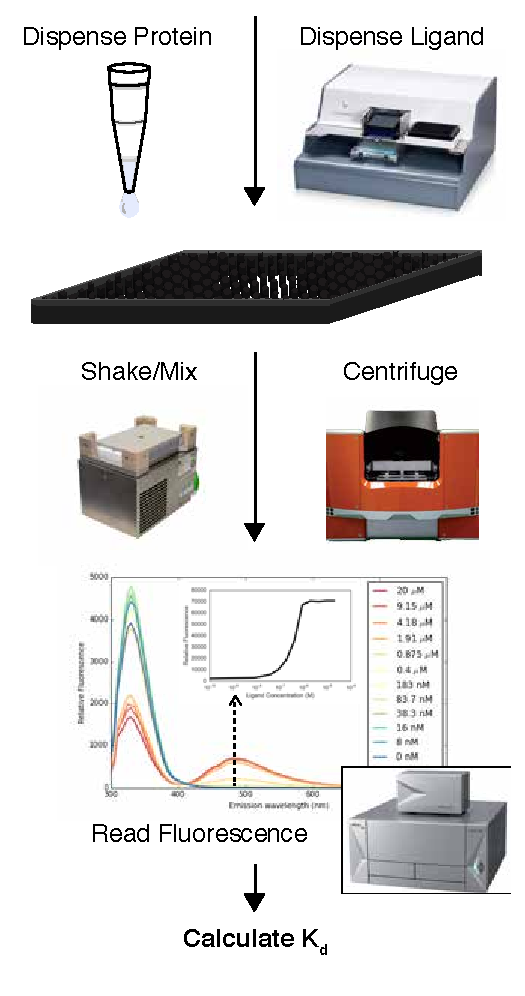
\includegraphics[width=0.9\textwidth]{Overview-v3.pdf}
\caption{\label{figure:example} {\bf Overview of the assay protocol.} 
This figure illustrates the assay protocol of this simple, direct, and automatable assay for kinase inhibitor binding affinities using fluorescent probe compounds.
}
\end{figure}


%%%%%%%%%%%%%%%%%%%%%%%%%%%%%%%%%%%%%%%%%%%%%%%%%%%%%%%%%%%%%%%%%%%%%%%%%%%%%%%%
% INTRODUCTION
%%%%%%%%%%%%%%%%%%%%%%%%%%%%%%%%%%%%%%%%%%%%%%%%%%%%%%%%%%%%%%%%%%%%%%%%%%%%%%%%

\section*{Introduction}
\label{section:introduction}

Wolf chartreuse beard ~\cite{levinson_structural_2012}, paleo bushwick locavore tumblr selvage health goth narwhal post-ironic meggings cronut DIY etsy. 
Tote bag viral craft beer migas, brooklyn keffiyeh shabby chic wayfarers godard scenester affogato pabst. 
Humblebrag chartreuse schlitz, post-ironic wolf ethical narwhal salvia everyday carry gastropub venmo kale chips. You probably haven't heard of them cornhole tilde readymade mixtape irony. 
Sriracha occupy yuccie, green juice roof party fap tumblr hammock mumblecore ramps pabst. Artisan listicle truffaut kogi, shabby chic kombucha distillery etsy cronut +1 pabst mustache VHS vinyl green juice. 
Before they sold out brooklyn yuccie, gluten-free sriracha lumbersexual four loko kombucha semiotics letterpress biodiesel kale chips art party normcore slow-carb.

%%%%%%%%%%%%%%%%%%%%%%%%%%%%%%%%%%%%%%%%%%%%%%%%%%%%%%%%%%%%%%%%%%%%%%%%%%%%%%%%%%%%%%%%%%%%%%%%%%%%%
% Methods
%%%%%%%%%%%%%%%%%%%%%%%%%%%%%%%%%%%%%%%%%%%%%%%%%%%%%%%%%%%%%%%%%%%%%%%%%%%%%%%%%%%%%%%%%%%%%%%%%%%%%
\section{Methods}

These are the Methods.

Wolf chartreuse beard, paleo bushwick locavore tumblr selvage health goth narwhal post-ironic meggings cronut DIY etsy. 
Tote bag viral craft beer migas, brooklyn keffiyeh shabby chic wayfarers godard scenester affogato pabst. 
Humblebrag chartreuse schlitz, post-ironic wolf ethical narwhal salvia everyday carry gastropub venmo kale chips. You probably haven't heard of them cornhole tilde readymade mixtape irony. 
Sriracha occupy yuccie, green juice roof party fap tumblr hammock mumblecore ramps pabst. Artisan listicle truffaut kogi, shabby chic kombucha distillery etsy cronut +1 pabst mustache VHS vinyl green juice. 
Before they sold out brooklyn yuccie, gluten-free sriracha lumbersexual four loko kombucha semiotics letterpress biodiesel kale chips art party normcore slow-carb.

%%%%%%%%%%%%%%%%%%%%%%%%%%%%%%%%%%%%%%%%%%%%%%%%%%%%%%%%%%%%%%%%%%%%%%%%%%%%%%%%%%%%%%%%%%%%%%%%%%%%%
% Results
%%%%%%%%%%%%%%%%%%%%%%%%%%%%%%%%%%%%%%%%%%%%%%%%%%%%%%%%%%%%%%%%%%%%%%%%%%%%%%%%%%%%%%%%%%%%%%%%%%%%%
\section{Results}

These are the Results.

Wolf chartreuse beard, paleo bushwick locavore tumblr selvage health goth narwhal post-ironic meggings cronut DIY etsy. 
Tote bag viral craft beer migas, brooklyn keffiyeh shabby chic wayfarers godard scenester affogato pabst. 
Humblebrag chartreuse schlitz, post-ironic wolf ethical narwhal salvia everyday carry gastropub venmo kale chips. You probably haven't heard of them cornhole tilde readymade mixtape irony. 
Sriracha occupy yuccie, green juice roof party fap tumblr hammock mumblecore ramps pabst. Artisan listicle truffaut kogi, shabby chic kombucha distillery etsy cronut +1 pabst mustache VHS vinyl green juice. 
Before they sold out brooklyn yuccie, gluten-free sriracha lumbersexual four loko kombucha semiotics letterpress biodiesel kale chips art party normcore slow-carb.

%%%%%%%%%%%%%%%%%%%%%%%%%%%%%%%%%%%%%%%%%%%%%%%%%%%%%%%%%%%%%%%%%%%%%%%%%%%%%%%%
% FIGURE TWO: COMPLEX SPECTRA
%%%%%%%%%%%%%%%%%%%%%%%%%%%%%%%%%%%%%%%%%%%%%%%%%%%%%%%%%%%%%%%%%%%%%%%%%%%%%%%%

\begin{figure*}[t]
\includegraphics[width=0.9\textwidth]{SpectraAssay-v3.pdf}
\caption{\label{figure:example} {\bf Example spectra of complex fluorescence when varying ligand concentration.} 
Here it is clear how saturation binding curves from which ligand binding affinities can be calculated can be measured using the fluorescence of the complex of kinases with fluorescent ligands like bosutinib.
}
\end{figure*}

%%%%%%%%%%%%%%%%%%%%%%%%%%%%%%%%%%%%%%%%%%%%%%%%%%%%%%%%%%%%%%%%%%%%%%%%%%%%%%%%
% FIGURE THREE: COMPETITION ASSAY
%%%%%%%%%%%%%%%%%%%%%%%%%%%%%%%%%%%%%%%%%%%%%%%%%%%%%%%%%%%%%%%%%%%%%%%%%%%%%%%%

\begin{figure}[tbp]
\includegraphics[width=0.9\textwidth]{Abl_Gef_Ima_grant.pdf}
\caption{\label{figure:example} {\bf Competition assays expand the relevance of this assay to innumerable other kinase inhibitors.}
Here imatinib is used to compete off the fluorescent ligand gefitinib. Thus binding affinities can be measured for even non-fluorescent ligands, expanding the applicability of this simple, direct, cheap, and automatable assay to innumerable other kinase inhibitors.
}
\end{figure}

%%%%%%%%%%%%%%%%%%%%%%%%%%%%%%%%%%%%%%%%%%%%%%%%%%%%%%%%%%%%%%%%%%%%%%%%%%%%%%%%
% ACKNOWLEDGMENTS
%%%%%%%%%%%%%%%%%%%%%%%%%%%%%%%%%%%%%%%%%%%%%%%%%%%%%%%%%%%%%%%%%%%%%%%%%%%%%%%%

\section*{Acknowledgments}

We are grateful to many people.
JDC acknowledges a Louis V.~Gerstner Young Investigator Award, NIH core grant P30-CA008748, and the Sloan Kettering Institute for funding during the course of this work.

%%%%%%%%%%%%%%%%%%%%%%%%%%%%%%%%%%%%%%%%%%%%%%%%%%%%%%%%%%%%%%%%%%%%%%%%%%%%%%%%
% BIBLIOGRAPHY
%%%%%%%%%%%%%%%%%%%%%%%%%%%%%%%%%%%%%%%%%%%%%%%%%%%%%%%%%%%%%%%%%%%%%%%%%%%%%%%%

\bibliographystyle{prsty} 
\bibliography{manuscript}

\end{document}